
\chapter{Proposed Method}\label{ch:method}

In this section we dervive anomaly detection method based on spectral decomposition
of time-domain signal.
Our goal is to involve statistical analysis of the frequency components of a 
time-domain signal for detection of the malicious behavior.
%\emph{tunneling protocol} %malicous traffic
%in an application layer as well as 

On the high-frequency scale (sample rate our method ought to be capable of detection of the
\emph{tunneling protocols} in application layer, while on the very low frequency scale 
our method is intended to be capable to detect anomalous behavior in wider time contexts.
The sample reate is induced by data format in use. Data providing traffic flow statistic
alread has been sampled at very low rate (e.g. $s=0.0033Hz$) and thus it is not possible
to analyze higher frequencies. The frequency scale is generaly a tradeoff between
computational comlexity and the needed resolution.

Tunneling protocol refer to encapsulation of one network 
protocol in payload of the other. By using tuneling protocol a malicious agent can 
transfer data  belonging to prohibited protocol over a network, bypassing 
a security policies. Our hypotesis is that application protocol imprints 
specific pattern in a power spectral density distribution. If the tunneling protocol 
is in use, these patterns ought to be different and anomalous behavior can be detected.

The periodicity can be analyzed on different scales, while tunneling protocol
violates normal pattern on higher frequency scales, we are also concerned about anomalous
patterns in very low frequency scales. This other patterns come up not of violation 
of the standard protocols, but of departure from the typical behavior or the habits. 
E.g. an mallware communicating with the remote server using the HTTP protocol 
does not violate the application protocol. 
But by exchanging information in regular manner, not depending on time of the day,
its behavior will be distint from the behavior of the typical web user who uses the network
in a way, periodic manner.

\name{He et al.}~\cite{he2004spectral} showed that the different layers of the network
protocols inprint distinct patterns in a power spectral density distribution. 
Further work of \name{Chen} and \name{Hwang}~\cite{chen2007spectral}
used the features derived %TODO use better word
from frequency spectrum to classify malicious and normal traffic.
They noticed that transport protocols (transmission control protocol --
TCP and user datagram protocol - UDP) 
have distinct power spectral density distribution. 
They exploited this property to identify low-rate denial-of-service (DoS)
attacks on TCP protocol. %TODO on TCP protocol?
%an reduction of service (RoS) attacks.
%TODO more writing about features used
In %this and future work %\cite{} 
their work they focused on reduction-of-service (RoS) attack.
The RoS attack unlike denial-of-service (DoS) attack does not attempt to completely deny the
service by throttling the resources using a fake requests, but the attacker`s focus is on 
reduction of the quality (e.g. prolong the response times) 
by using small ammount of the requests. 
Due to low traffic during attack, RoS attacks are hard to detect with volume-based methods.

%\name{Wright et al.}~\cite{wright2006inferring} researched methods based on 
%hidden Markov models to classify different application protocols embeded in 
%encrypted application layer.
%They developed classification method, able to classify different 
%application protocols multiplexed in single encrypted packet flow.
%\name{Dusi et al.} brought an statistical approach 
%to detect an tunnel inside application layer.
%In ~\cite{dusi2009tunnel}  they described different tunneling techniques and designed 
%statistical pattern recognition classifier to identify them.

Even though it is not possible to analyze payload of particular packets in 
ecrypted connection, it is possible to observe the time of the packet transit, 
its size, direction, source and destination endpoint, etc. 
This data is denoted as packet traces and it is extracted from unencrypted 
part of the packet. 
The goal is to develop feature creation and pattern recognition method for 
the network packet traces involving spectral analysis.
The method is supposed to detect tunneling protocols only by observation 
of the packet traces.

\section{Data Collection}\label{sec:collect}

The input data for our method consists of a timestamped \emph{packet traces} or a
timestamped \emph{traffic flow} statistics. 

Both can be obtained by capturing
network packet headers. While first one stores each packet (or the packet header)
as a single record,
other one contains total count of the packets and ammount of bytes for 
related sequence of the packets. Relation between packets is determined depending 
on the traffic flow protocol. E.g. for Transmission Control Protocol (TCP) relation is 
determined using following information: capturing interface, source and destination IP address,
source and destination port. 
%
%or Cisco standard \emph{NetFlow}%
%\footnote{
%Cisco standard definest one record (a flow) in Netflow format as a unidirectional sequence of
%packets that share following values: ingress interface; source IP address; destination 
%IP address; IP protocol; source port for UDP or TCP, 0 for other protocols;
%destination port for UDP or TCP, type and code for ICMP, or 0 for other protocols;
%type of service (TOS).
%} 
%protocol. As NetFlow datasets contains only statistics of particular network packet flows, 
%it can be generated from the packet trace data. In practice the NetFlow data is generated by 
%network active components as firewals, routers or swithes. 
%

Due to differences in described formats, we extract following attributes 
from packet trace or traffic flow data in our experiments, 
to allow usage of unified processing methods:
\begin{itemize}
	\item packet or packet flow \emph{timestamp}, i.e. the time when the (first) packet passed
	trought the capturing gateway,
	\item \emph{flow 5-tuple} -- i.e. tranmission \emph{protocol} speciffication and identification of 
	source and destination endpoint
	(e.g. for the TCP or the UDP protocols it is \emph{address} and \emph{port}, 
	\emph{destination address}  and \emph{port}),
	\item \emph{size} of packet`s payload or \emph{total size} of the packets in case of flow data,
	\item \emph{count} of the packets (for packet trace data it is always one),
	\item \emph{direction}%
	\footnote{%
		We embed \emph{direction information} 
		into the \emph{size} parameter using negative size  
		if packets travel from destination to source and otherwise positive.%
	} %
	with respect to initial packet whithin given flow,
\end{itemize}

We define source endpoint as the endpoint that initiates connection and the destination edpoint 
as the endpoint that  accepts the connection. %TODO what?
Inbound and outbound packets are distinguished
by direction attribude. 

We further require that traffic flow data are allways captured periodically in defined time span.
We can look at this process as a sampling process. We consider the flow capturing period
is lower bound for the sampling period. This can of course cause alliasing as the original
signal contains higher frequency components than the sampling frequency induced by data capturing 
process. For packet trace data there is no upper bound on the sampling frequency induced by 
capturing process, but higher sampling frequency raises the memory and processig time requirements.

For purposes of evaluation (see sections~\ref{subsec:eval} and~\ref{subsec:roc}) data labeling 
must be provided.
The label is basically and mark that identifies arbitrary flow and groups  several flows into
classes. For purposes of anomaly detection two classes are expected: \emph{normal}, \emph{anomalous}.
However it can by complicated when discrimination between specific classes is needed.
As we are exploiting properties of HTTP protocol, we take in account following classes: 
\emph{http normal}, \emph{http tunnel} and \emph{http mallware}, which are a subset of all possible 
classes available in traffic.
The process of labeling of the data is dscribed in section~\ref{subsec:labeling}.

\section{Feature Creation}

\subsection{Stochastic process}
% TODO some flesh here

For a specified flow $f$ the packet arrival process $x_f\left[t\right]$ 
(or simply \emph{packet process})  is defined as a count of packet arrivals 
at given timespan $I = \left\langle \frac{t}{s}, \frac{t+1}{s} \right)$:
\begin{equation}\label{packetprocess}
\begin{split}
	 x_f\left[t\right] = \left| 
	\left\lbrace p : f = flow(p) \wedge time(p) \in I \right\rbrace \right|\\
	\forall t \in \mathbb{N}\, ,
\end{split}
\end{equation}
where $s$ is the sample rate, function $flow(p)$  yields the \emph{flow} 5-tuple 
and function $time(p)$  yields the \emph{timestamp} of given packet $p$. 
We can also define packet process for inbound and outbound flows separately:
\begin{equation}\label{xpacketprocess}
\begin{split}
  x_{f,d}\left[t\right] = \left| 
  \left\lbrace p : flow(p) = f \wedge dir(p) = d \wedge time(p) \in I  \right\rbrace \right|\\
  \forall t \in \mathbb{N}\, ,
\end{split}
\end{equation}%
where $dir(p)$ yields a direction of the packet. 

Note that we will refer to single flow and to avoid confusion
we will denote packet process as $x$ and the inbound and
outbound packet processes as $x_{in}$ and $x_{out}$  in equations. 
%\footnote{
%This is very important formula, we need to focus on it; according 
%to \emph{Dusi et al.}~\cite{dusi2009tunnel}
%zero-length packets are ulikely to be induced by application, 
%so we can exclude them here; in addition
%they extract incomming and outgoing  stream separately -- 
%I think it is good idea to work with in- and out- streams separately 
%and compute cross-correlation function instead of auto-correlation function.
%The idea of usage I/O cross-correlation function $R_{io}\left(\tau\right)$ 
%instead of auto-correlation is that $R_{io}\left(\tau\right)$ (at the specific 
%time-lag $\tau$) would enforce the typical request-response round-trip. 
%Questionable is, how to physically interpret the resulting spectral components 
%and if the Wiener-Kitchin theorem is applicable.
%}


\subsection{Spectral density estimator}\label{sec:psd}
% TODO some flesh here -  more about wiener-kitchine theorem and sampling theorem

According to a Wiener–Khinchine %TODO reference
theorem the power spectral density $S_{xx}(f)$ (PSD) of the wide-sense stationary 
stochastic process is obtained by application of discrete-time 
Fourier transform $\mathcal{F}_{\cdot}(\omega)$ on autocorrelation function 
of the packet process $R_{xx}\left[\tau\right]$:

\begin{equation}\label{eq:corr}
R_{xx}\left[\tau\right] = E[x\left[t\right]x\left[t+\tau\right]]\, , 
\end{equation}

\begin{equation}\label{eq:psd}
\begin{split}
S_{xx}(\omega) = \mathcal{F}_{R_{xx}}\left(\omega\right) = \sum_{\tau=-\infty}^{\infty} 
\left( R_{xx}\left[\tau\right] \exp\left( -\imath \omega\tau \right)\right) \\ 
\forall f \in \left\langle -\frac{s}{2},\frac{s}{2} \right\rangle\, , 
\end{split}
\end{equation}

where $\tau$ is the time-lag, $E\left[\cdot\right]$ is expected value of a random variable, $\imath$
is the imaginary unit and $\omega$ is the angular frequency $\omega= 2\pi f$. 
%The autocorrelation function is capable of enforcing periodicity. %TODO really?

Analyzing the inbound and outboud packet process can lead to definition of the cross spectral
density\cite{penny2000signal}.
As the power spectral density is Fourier tranform of the autocorrelation function of the 
stochastic process cross spectral density is the fourier transform is the fourier transform
of the cross-correlation function of two stochastic processes. The cross spectral density is
complex as because the cross-correlation function is not symmetric. 
For inbound and outbound packet process we define cross-correlation function $R_{io}$ 
as well as the cross-spectral density $S_{io}$ as follos:

\begin{equation}\label{eq:xcorr}
R_{io}\left[\tau\right] = E[x_{in}\left[t\right]x_{out}\left[t+\tau\right]]\, , 
\end{equation}

\begin{equation}\label{eq:xpsd}
\begin{split}
S_{io}(\omega) = \mathcal{F}_{R_{io}}\left(\omega\right) = \sum_{\tau=-\infty}^{\infty} 
\left( R_{io}\left[\tau\right] \exp\left( -\imath \omega\tau \right)\right) \\ 
\forall f \in \left\langle -\frac{s}{2},\frac{s}{2} \right\rangle\, , 
\end{split}
\end{equation}

Equations (\ref{eq:corr}), (\ref{eq:psd}), (\ref{eq:xcorr}) and (\ref{eq:xpsd}) 
hold under assumption that packet process is \emph{wide-sense stationary random proces}.
This asssumption seems to be false for infinite time span in network traffic.
Furthermore the time span is usually limited to finite number of samples.
For practical reasons we involved an \emph{windowing function} $w(n)$ and 
\emph{discrete Fourier transform} instead of discrete-time Fourier transform. 
The simplest windowing function -- a rectangular windowing is defined as follows:
\begin{equation}
w(n) = \left\lbrace \begin{array}{l} 
1, \mbox{ if } n\in \left\langle 0, M \right) \\ 
0, \mbox{ otherwise} \end{array}\right. \,.
\end{equation}
Windowing function is nonzero inside specified interval $\left\langle 0, M \right)$ 
otherwise it is zero (see fig.~\ref{fig:windowing}). 

\begin{figure}[h!]%
  \centering
  \includegraphics[width=0.5\textwidth]{img/windowing}
  \caption{\small Rectangular and hamming windowing function for M = 250}
  \label{fig:windowing}
\end{figure}

Parameter  $M$ is length of sub-sequence selected from packet arrival proces. 
If the parameter $M$ is too high the packet proces is unlikely to be stationary, 
on the other hand selecting too low value causes spectral leakage, i.e. the energy 
of the main lobe of a spectral response "leaks" to the sidelobes distorting the 
spectral responses~\cite{kay1981spectrum} 
(fig.~\ref{fig:leakage_rect_1000},~\ref{fig:leakage_rect_25}). 

\begin{figure}[h!]%
  \centering
        \begin{subfigure}[b]{0.5\textwidth}
                \centering
                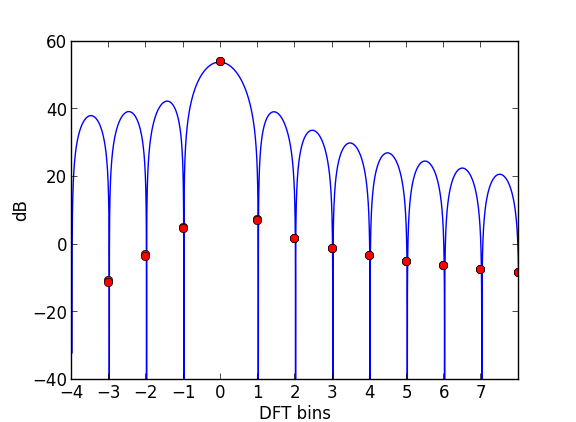
\includegraphics[width=\textwidth]{img/leakage_rect_1000}
                \caption{\small rectangular, $M=1000$}
                \label{fig:leakage_rect_1000}
        \end{subfigure}%
        ~ \begin{subfigure}[b]{0.5\textwidth}
                \centering
                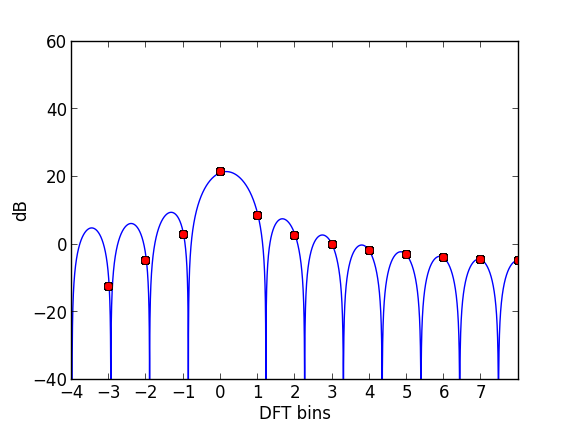
\includegraphics[width=\textwidth]{img/leakage_rect_25}
                \caption{\small rectangular, $M=25$}
                \label{fig:leakage_rect_25}
        \end{subfigure}%
  \caption{\small Detail of the discrete-time Fourier transform (DTFT) of a sinusoid 
  with rectangular  windowing.
  The unit on x-axis is an Discrete fourier transform (DFT) bin.
  The red dots show values returned by DFT. It is visible that for decreased widow
   size (fig.~\ref{fig:leakage_rect_25}) the distortion is higher. Note that this is 
   artifact of the selected windowing and the period of the sinusoid.}
  \label{fig:leakage_rect}
\end{figure}

We iteratively apply windowing function to the whole sequence of samples generating 
non-overlapping adjancent sequence of windows. 
We identify the particular window in this sequence with upper index -- 
e.g. $S_{xx}^i$ is a power spectral density function of an $i$-th window.
Thus, we rewrite equations (\ref{eq:corr}) and (\ref{eq:psd}) for non-overlapping 
windows as follows:
\begin{equation}\label{eq:corr2}
R_{xx}^i\left[m\right] = \frac{1}{M} \sum_{t=0}^{M}
 x\left[t+iM\right]x\left[t+m+iM\right] \, , 
\end{equation}
\begin{equation}\label{eq:psd2}
\begin{split}
S_{xx}^i(k) = \mathcal{F}_{R_{xx}^i}\left(k\right) = \sum_{m=0}^{M-1}
\left( R_{xx}^i \left[m\right] w(m) \exp\left( -\imath 2\pi m\frac{k}{M} \right)\right)\\
\forall k \in \left\{ 0,1,2,...,M-1 \right\}\, . 
\end{split}
\end{equation}
and similarly for cross spectral density:
\begin{equation}\label{eq:xcorr2}
R_{io}^i\left[m\right] = \frac{1}{M} \sum_{t=0}^{M} 
 x_{in}\left[t+iM\right]x_{out}\left[t+m+iM\right] \, , 
\end{equation}
\begin{equation}\label{eq:xpsd2}
\begin{split}
S_{io}^i(k) = \mathcal{F}_{R_{io}^i}\left(k\right) = \sum_{m=0}^{M-1}
\left( R_{io}^i \left[m\right] w(m) \exp\left( -\imath 2\pi m\frac{k}{M} \right)\right)\\
\forall k \in \left\{ 0,1,2,...,M-1 \right\}\, . 
\end{split}
\end{equation}
Note that the windowing function is inherent in equations (\ref{eq:corr2}) and (\ref{eq:psd2})
by using limitted ranges of sumation, and domain of definition of the power spectral density.

\begin{figure}[h!]%
  \centering
        \begin{subfigure}[b]{0.5\textwidth}e
                \centering
                \includegraphics[width=\textwidth]{img/leakage_hamming_1000}
                \caption{\small hamming, $M=1000$}
                \label{fig:leakage_hamming_1000}
        \end{subfigure}%
        ~ \begin{subfigure}[b]{0.5\textwidth}
                \centering
                \includegraphics[width=\textwidth]{img/leakage_hamming_25}
                \caption{\small hamming, $M=25$}
                \label{fig:leakage_hamming_25}
        \end{subfigure}%
  \caption{\small Detail of the discrete-time Fourier transform (DTFT) of a sinusoid 
  with hamming windowing.
  The unit on x-axis is an Discrete fourier transform (DFT) bin.
  The red dots show values returned by DFT. It is visible that for decreased widow
   size (fig.~\ref{fig:leakage_hamming_25}) the distortion is higher.}
  \label{fig:leakage_hamming}
\end{figure}

By involving windowing function we introduced
\emph{spectral leakge}. Use of apodization function, e.g. \emph{Hamming} %TODO explain 
(see fig.~\ref{fig:leakage_hamming_1000} and~\ref{fig:leakage_hamming_25}),
%or \emph{Hamming} (\ref{eq:hamm}) 
could be appropiate in decreasing leakage:
%\begin{equation}\label{eq:hann}
%w(n) = \left\lbrace \begin{array}{l} 
%0.5\left(1 - \cos \left ( \frac{2 \pi n}{N-1} \right) \right), \mbox{ if } n\in \left\langle 
%0, M \right) \\ 0, \mbox{ otherwise} \end{array}\right. \,.
%\end{equation}
\begin{equation}\label{eq:hamm}
w(n) = \left\lbrace \begin{array}{l} 
0.54 - 0.46\cos \left ( \frac{2\pi n}{N-1} \right), \mbox{ if } n\in \left\langle 0, M \right) \\
 0, \mbox{ otherwise} \end{array}\right. \,.
\end{equation}
The hamming window still allows to leak the power to nearby DFT bins as the
main lobe is wider, but the attenuation of in side lobes is higher.
Even the hamming window cannot provide good results for the low values of the $M$ 
parameter. In addition there is allways tradeoff between effective bandwidth and
sidelobe attenuation. \name{Yoon} et al.~\cite{yoon2009butterworth} windowing technique 
involving a Buttleworth filter to overcome the problems with reduction of bandwith 
while elevating sidelobe attenuation.

The sampling rate $s$ must be selected according to the Nyquist theorem. 
Too low value entails aliasing%
\footnote{
    The aliasing is caused by folding of the frequencies above Nyquist frequency
    $\frac{s}{2}$ symmetrically below this frequency. 
    To properly reconstruct the signal that contain no frequency higher than $f_{max}$ 
    the sample rate is bounded by $s > 2f_{max}$.
}%
, while too high value incurs data storage and processing overhead. 
%\subsection{Pattern definition}
By application of the Fourier transform original features has been mapped into new space.
We denote features in new space as \emph{spectral components} (or \emph{frequency components}).
Temporal context of the features has been altered. 
In new feature space the temporal context is determined by sequence
of the detection windows of size $M$. 
%At the level of the detection window a temporal notion is decomposed 
%into tuple of temporal functions parametrised by \emph{spectral components}.

The determination of the changes in spectrum in local time context is related to short-term
Fourier analysis or short-term Fourier transform. Whereas this approach introduces
resolution problems wavelet transform or multiresolutional analysis can be used for
time-frequency analysis. We are not concerned with temporal context at this point.
Although temporal aspect is still present it has not been used in further analysis 
in present work. Anomalies in new feature space are thus regarded to as \emph{point anomalies}. 

\subsection{Parameters}

There are few parameters affecting generation of the  features: %TODO what?
the sample rate $s$ and the window length $M$. 
In addition, \emph{spectral components} can be subject to further feature extraction 
comprising combination of extisting features or discarding irrelevant, 
redundant  or noisy%
\footnote{
    In case of low signal-to-noise ratio, a feature is typically not usefull 
    for discriminative outcome.
} %
ones using data-mining methods or based on the empirical domain knowledge.

This aspects and process of seeking of proper parameters are subject of further 
research and they are discussed in \emph{chapter~\ref{ch:experiments}}. 
Another apects related to searching for proper paramters (statistical 
validation procedure) are discussed in \emph{subsection~\ref{sec:val}}.

\section{Model Estimation and Anomaly Detection}

In order to detect anomalies a model of normal or anomalous behavior or even both
must be constructed. The na\"ive approach is to estimate an multivariate gaussian 
model under assumption of \emph{central limit theorem}. This approach encounters 
serveral problems. The most notable is the curse of dimensionality - 
an phenomena occuring when analyzing data in high-dimensional spaces.
The statistical view on this problem is that by applying tranformations 
to create high-dimensional features the data become sparse. It is problem to 
have statisticaly significat outcome as the amount data needed is emerging
exponentially with dimensionality. 

Another facet of mentioned na\"ive approach is assuption of central limit theorem, 
meaning that the data instances are independent and identically distributed. 
In addition, to obtain an sound and reliable result sufficient number of data instances 
must be present. This is often problem as the data instances that are related to anomalies 
are less common in data. Additional data instances can be artificially simulated in order 
to enable ability to construct an reliable model. Introducing  systmatic errors during 
simulation can lead to biased model estimator. %In addition simulation of annomalous
%intances can bias the model as it affects the extent in which are such instances present in data.

The solution to course of dimensionality is to reduce dimensionality of the feature space.
The reduction can be performed using  linear transformation. The goal is to find an 
linear basis such that the resulting data is denser and thus contains more information.
This idea is used by several linear dimensionality reduction techniques e.g. Principal 
Component Analysis (PCA).
We can also refer to finding manifold of denser data in original sparse feature space.
Reduction of dimensionality is then proces of estimation of topological properties of such 
manifold and the estimation of relations between data instances on the topological surface.
This technique is used in Kohonen maps (KM) or local linear  embedding (LLE) as the 
representatives of non-linear dimensionality reduction techniques.
 
Another approach is to use empirical domain knowledge to infer relations in the
data to perform transformation in lower dimansional space.

Spectral density of a signal in time domain represents continous decomposition of signal to
periodic components present in the original signal. Altought it is continous function in
practice only estimations are available. In section~\ref{sec:psd} we derived discrete
spectral density estimator based on auto-correlation function. 
The analyzed signal is connected to stochastic processes
that occur in computer network. The frequency distribution of signals in such a system is 
affected by many attributes. Our assumption is that te stochastic processs in computer network
are stationary. It is false thougth to try to pick an specific characteristic frequency component
and treat it as a discriminative feature for specific undelaying process. As example when an 
saturated link is changing its speed the characteristic frequency changes as well, it has been
explored by \name{He} et al. in~\cite{he2004spectral}.

\name{Chen} et al.~\cite{chen2007tcp} presented an approach where modeled distribution
of a standard deviation over spectral densities and also multivariate distribution over
frequency bands. Their model used diagonal covariance matrix. They performed hypotesis 
testing in order to classify an cut-off specific type of denial-of-service (DoS) attacks.
In present work we consider above methods of statistical analysis of 
the spectral density and go further.

In following subsections we introduce proposed 
dimensionality reduction and model estimation methods.

\subsection{Feature Extraction}

At first it should be noted, that the Fourier transform of the autocorrelation function 
is real and symmetric. The reason is that periods in input data turn into positive and negative
components. Negative components contains same information as the postive. 
First step in reduction of the dimensionality is discarding redundant features.

\paragraph*{Band Filters.}
Other possible linear transformation is frequency-band filtering. 
The transformation matrix used to perform band-filtering is sparse and easy to 
interpret by human analyst. Transformation is basically dot product:
\begin{equation}
\mathbf{X}_t = \mathbf{X}\mathbf{A} \;,
\end{equation}
where $\mathbf{A}$ is $n\times m$ transformation matrix, $\mathbf{X}$ is original 
$n$-dimensional sample of length $N$ ($N\times n$ matrix) and $\mathbf{X}_t$ is  
new sample of $m$ dimensions; data instances are row vectors.
Recall the equation (\ref{eq:psd2}); the Power Spectral Densities $S_{xx}^i\left(k\right)$ 
are the element of matrix $X$ at $k$-th row and $i$-th column.

By transformation matrix 
\begin{equation}
\mathbf{A} = 
\begin{bmatrix}
  1 & 0 \\
  1 & 0 \\
  0 & 1 \\
  0 & 1
 \end{bmatrix}  \;
\end{equation}
we provide sum of the lower half and the upper half of the features:
\begin{equation} 
 \begin{bmatrix}
  x_{11} & x_{12} & x_{13} & x_{14}  \\
  x_{21} & x_{22} & x_{23} & x_{24}  \\
  \cdot & \cdot &\cdot & \cdot  \\
  \cdot & \cdot &\cdot & \cdot  \\
  x_{N1} & x_{N2} & x_{N3} & x_{N4} 
 \end{bmatrix}
\begin{bmatrix}
  1 & 0 \\
  1 & 0 \\
  0 & 1 \\
  0 & 1
 \end{bmatrix}  \;= \;
 \begin{bmatrix}
  x_{11} + x_{12} & x_{13} + x_{14}  \\
  \cdot & \cdot &  \\
  \cdot & \cdot &  \\
  x_{N1} + x_{N2} & x_{N3} + x_{N4} 
 \end{bmatrix}
\end{equation}
In similar manner band filters can be constructed in higher dimmensional space.


%TODO formula for band filter based on itervals
\paragraph*{Principal Component Analysis.}
Different approach is to involve a Principal Component Anaysis (PCA). 
The PCA is used to perform othogonal transformation to convert a set of correlated data instances into 
another set that is uncorrelated. The components in new feature space are ordered  
such that the first component has the largest variance, %TODO link to paper on PCA
%TODO image of PCA

\begin{figure}[h!]%
  \centering
  \includegraphics[width=0.5\textwidth]{img/pca}
  \caption{\small Principal component analysis}
  \label{fig:pca}
\end{figure}

i.e. the components are ordered from the most informative to the least informative ones.
As the variance is decreasing data is more sparse and less informative.
In our analysis we use first $m$ components to reduce dimensionality and enforce
density of the data. Each compoenent is represented by vector in othogonal transformation basis
called eigenvector denoted $e_i$ for $i$-th component.
An scalar value $\lambda_i$ representing an variance of $i$-th component called eigenvalue and it 
is associated with each eigenvector.
A method of computation of the eigenvectors $e_i$ and eigenvalues $\lambda_i$ based on covariance matrix
decomposition is defined as follows: Given a sample $\mathbf{X}$ ($N\times n$ matrix), 
compute sample mean vector $\overline{\mathbf{x}}$ and sample covariance matrix $\mathbf{S}$:
\begin{equation}\label{eq:sampmean}
	\overline{\mathbf{x}} = \frac{1}{N} \sum_{i=1}^N \mathbf{x_i} \;,
\end{equation}
\begin{equation}\label{eq:sampcov}
	\mathbf{S} = \frac{1}{N-1} \sum_{i=1}^N  \left(\mathbf{x_i} - \overline{\mathbf{x}} \right) 
	\left(\mathbf{x_i} - \overline{\mathbf{x}} \right)^\top \;.
\end{equation}
Eigenvectors an eigenvalues are then solution to equation:
\begin{equation}
	\mathbf{S}e = \lambda e \;.
\end{equation}
Ordering eigenvectors and eigenvalues such that $\lambda_1 \geq \lambda_2 \geq \dots \lambda_n$ and
selecting first $m$ eigenvectors results in linear transformation:
\begin{equation}
	\mathbf{E} = \left[ e_i^\top \right]_{i=1}^m\;,
\end{equation}
\begin{equation}
	\mathbf{X_t} = \mathbf{E} \mathbf{X} \;.	
\end{equation}

The  portion of variance explained by each of the components included in transformed sample $X_t$
is and quantitative measure $q$ of the model, defined as:
\begin{equation}
	q_m = \frac{\sum_{i=1}^m\lambda_i}{\sum_{j=1}^n\lambda_j} 
\end{equation}

To obtain an effective transformation a ratio $q_m$ should fall off rapidly  for sufficiently small number
of retained eigenvectors $m$. For example in image processing only first $3-5$ eigenvectors are 
significant while the input data (images) can have hundreds of dimensions.
Advantage of using PCA transformation to frequency components is that it introduces new feature space
that is much more informative, than the original feature space. Drawback is that the orthogonal basis 
is harder to explain.

%\paragraph*{H. Ringberg, 
%Sensitivity of PCA for traffic anomaly detection}
%\cite{ringberg2007sensitivity}
%Detecting anomalous traffic is a crucial part of managing IP networks. In recent years, network-wide anomaly detection based on Principal Component Analysis (PCA) has emerged as a powerful method for detecting a wide variety of anomalies. We show that tuning PCA to operate effectively in practice is difficult and requires more robust techniques than have been presented thus far. We analyze a week of network-wide traffic measurements from two IP backbones (Abilene and Geant) across three different traffic aggregations (ingress routers, OD flows, and input links), and conduct a detailed inspection of the feature time series for each suspected anomaly. Our study identifies and evaluates four main challenges of using PCA to detect traffic anomalies: (i) the false positive rate is very sensitive to small differences in the number of principal components in the normal subspace, (ii) the effectiveness of PCA is sensitive to the level of aggregation of the traffic measurements, (iii) a large anomaly may in advertently pollute the normal subspace, (iv) correctly identifying which flow triggered the anomaly detector is an inherently challenging problem.


\paragraph*{Moment Estimate Matrix.}
Finally, instead of analysing components individually, an statistical agregation can be applied, e.g.
variance estimation of the individual spectral vectors. Extending this approach can lead in
construction of new $k$-dimensional feature space using first $k$ moments, i.e. the mean, variance,
skewness and kurtosis of the spectra.

An unbiased estimator of the $k$-th moment ${\mu^{(k)}}$ is a sample $k$-th moment 
$\overline{\mu}^{(k)}$:
\begin{equation}
\overline{\mu}^{(k)} = \frac{1}{n} \sum_{i=1}^n\mathbf{x}_i^k\;,
\end{equation}
applied on sample $\mathbf{X} = \left[ \mathbf{x}_1, \mathbf{x}_2, \dots, \mathbf{x}_n \right]$ 
drawn from population ($\mathbf{x}_i$ are column vectors $N\times 1$).
In our case the sample is the finite set of the spectral components that are drawn from 
infinite spectrum. A matrix of moment estimations $\overline{\mathbf{M}}$ of sample $X$ is 
then defined as:
\begin{equation}
	\overline{\mathbf{M}} = \left[ \overline{\mathbf{\mu}}^{(k)}\right]_{k=1}^m\;.
\end{equation}
Moments represents statistics that describe the shape of the distribution of a population.



\subsection{Model Fitting}

\paragraph*{Gaussian Model.}
As stated, we propose use of parametric model. Assuming central limit theorem a model ougth to be
$m$-dimensional Gaussian distribution $\mathcal{N}\left(\mu,\Sigma\right)$, where $\mu$ is the mean vector
and $\Sigma$ is the covariance matrix.  
%TODO formula for gaussian distribution
Values on diagonal of the matrix are variances of the particular features. 
Remaining values are covariances and for uncorrelated data they are equal to zero. 
 
Given the number of dimension $m$ of feature space,
number of free parameters when using full covariance matrix is $m+m^2$, while when reducing 
to diagonal matrix the count of the free parameters falls off to $2m$. 
It can be practical to assume that features are uncorrelated and retain only values on diagonal 
even if it is known that this asumption is false. It is because number of samples needed to accurately
estimate the model grows with count of the parameters. Reducing covariance matrix to diagonal 
will reduce size of data needed quadratically.

In estimation of parameters of the model one can involve \emph{Maximum Likelihood Estimates} (MLE).
%already introduced unbiased estimators -- an sample mean (\ref{eq:sampmean}) and sample covariance (\ref{eq:sampcov}). 
As this estimate is sensitive to presence of noise in data a robust estimator ougth to be taken in account.
Rousseeuw in~\cite{rousseeuw1984least} introduced Minimum Covariance Determinant estimator. The 
idea is to find an observations whose sample covariance has the smallest determinant. This subset is
then used to compute standard estimates of mean an covariance.

\paragraph*{Gaussian Mixture Model.}
By grasp of the central limit theorem we assume that when modeling a simple behavior captured by sample 
$\mathbf{X}$, the data instances of the samples are independent and idetically distributed (i.i.d.).
In case, the behavior is complex the sample $\mathbf{X}$ can be divided to $k$ equally distributed 
disjoint subsamples $\mathbf{X_i}$ in which the data instances can be assumed to be i.i.d.  
An attractor distribution in this case is countable mixture of Gaussian distributions
$Mix_{i=1}^k\left(\mathcal{N}\left(\mu_i,\Sigma_i\right)w_i\right)$, for each subsample $\mathbf{X_i}$, 
where $w_i$ is the weight of the distribution in mixture and it is proportional to cardinality of subsample
$\left| \mathbf{X_i} \right|$.
%TODO mixed gaussian

%TODO estimation of the model E-M

\subsection{Anomaly Score}

An anomaly score of test instance $\mathbf{x_t}$ is test statistics that is used 
to determine if the instance is anomalous or not. It is related to statistical hypothesis testing where
the null hypothesis $H_0$ is the conjecture that isntace is anomalous.

For example followig statistic is given by  Grubbs in~\cite{grubbs1969procedures}:
under assumption that instance is generated by a univariate gaussian distribution 
a $z$-statistic can be computed:
\begin{equation}
	{z} = \frac{{x_t}-\overline{{x}}}{{s}}\;, 
\end{equation}
where $x$ is test instance, $\overline{{x}}$ is sample mean and ${s}$ is standard deviation 
of the sample. A instance is declared anomalous if:
\begin{equation}
	{z} > \frac{N-1}{\sqrt{N}}\sqrt{\frac{t^2_{0.5\alpha/N,N-2}}{N-2+t^2_{0.5\alpha/N,N-2}}}\;,
\end{equation}
Where threshold $t^2_{0.5\alpha/N,N-2}$ it the value drawn of a Student`s $t$-distribution at significance level 
$0.5\alpha/N$. 
A variant for multivariate data uses a Mahalanobis distance as test statistic:
\begin{equation}
	y^2 = (\mathbf{x} - \overline{\mathbf{x}})\mathbf{S}^{-1}(\mathbf{x} - \overline{\mathbf{x}})^\top\;,
\end{equation}
where the $\overline{\mathbf{x}}$ is sample mean vector and $\mathbf{S}$ sample covariance matrix.
Same test, using $t$-distribution, is applied to test statistics $y$ as in case of $z$-statistic in Grubbs test.

Our proposal is to provide Mahalanobis distance as an raw anomaly score for further anomaly evaluation.
A discrimination threshold ougth to be estimated using an empirical validation on test sample.
 
\section{Parameter Selection and Empirical Evaluation}\label{sec:val}

The feature creation and model fitting procedures require proper parameter selection to accurately
estimate the model. The procedure for estimation a measure of fit has to be introduced.
Outcome of the anomaly detection technique based on statistical model uses model
to estimate anomaly score for a data instance.

\subsection{Stratified $k$-fold Cross Validation}

For estimation how accurately a model will perform in practice a cross validation technique has been developed.
The input to cross validation process is sample set, along with a labeling information. 
In one round, the cross validation involves partitioning sample set into complementary subsets, preforming analysis
and fitting the model on one set (training set) and validation of the model on the second set (testing set).
In order of reduce variability multiple rounds are needed.

In $k$-fold cross validation the sample is randomly  divided into $k$ disjoint subsamples of equal size. 
The cross validation round is then invoked $k$ times with each of the subsample used once as a testing set,
while the rest is used for fitting the model. When using stratified $k$-fold cross validation the folds are selected
such that the distribution of the labels in folds is uniform.

The output of the $k$-fold cross validation is set of $k$ partial outcomes. That can be averaged to produce
final outcome.

If we denote a measure of the model performance or the measure of fit  as $P$, 
the cross validation produces an estimate $P^*$ of the
expected performance $EP$. If cross validation is performed using multiple subsamples the values for $P^*$
will vary. An estimator $P^*$ is biased estimator for $EP$. The reason of bias is that training set is smaller
than the original sample and thus the estimated model is ``worse'' performing. 
For value $k$ equal to size of the sample, the bias is very small as allways one data instance is left out of 
training set. This approach uleashes huge computational overhead and it is rarely used.
As $P^*$ is always underestimate measure it is not a concern in many cases.
The much more concerns are due to its high variance. In case the variance is hight different
models are not comparable. This usually holds if the sample size is low.
In that case the evaluation process does not provide statistically sound and significant outcome.

\subsection{ROC curve}\label{subsec:roc}

For labelled data instances drawn from testing sample, an receiver operating characteristic 
(ROC curve) can be computed. 
In order to compute ROC curve an introduction of discrimination threshold on raw score 
is required. If a value of the raw score of a data instance is higher than discrimination 
threshold the instance is marked as anomalous. The discrimination threshold in conjunction 
with dataset labeling is used to compute true positive and false positive rates.
The ROC curve is plot of the true positive rate $r_{tp}$ vs. the false positive rate $r_{fp}$ 
while the threshold is varied.
The false positive rates and true positive rates are related to statistical hypotheses testing
where the null hypothesis ($H_0$) is the conjecture that given instance is anomalous.
Anomalous instance is also called ``positive''. Table~\ref{tbl:hypo} categorizes positive and
negative outcomes  with respect to validity of null hypothesis.

\begin{table}[h]
    \begin{center}
        \begin{tabular}{c|cc}
        	%& Sample is anomalous & Sample is normal \\ \hline
        	& Null hypothesis is true (P)	& Null hypothesis is false (N) \\ \hline
        	Reject null hypothesis & False negative (FN) & True negative (TN) \\
        	Fail to reject null hypothesis & True positive (TP) & False positive (FP) \\ %\hline
        \end{tabular}
    \end{center}
    \caption{\small Relations between true and false outcomes and the validity of hypothesis $H_0$.}
    \label{tbl:hypo}
\end{table}



Failure to detect anomalous instance is the false positive (FP) and correct detection is true positive (TP).
Given a testing sample set a false positive rate $r_{fp}$ is a proportion of false positives $n_{fp}$ vs.
all negative instances $n_{fp} + n_{tn}$:
\begin{equation}
	r_{fp} = \frac{n_{fp}}{n_{fp}+n_{tn}} \;,
\end{equation}
and the true positive rate (sensitivity) $r_{tp}$ is propotion of true positives $n_{tp}$ 
vs. all positive instances $n_{tp} + n_{fn}$:
\begin{equation}
	r_{tp} = \frac{n_{tp}}{n_{tp}+n_{fn}} \;.
\end{equation}

\begin{figure}[h!]%
  \centering
   \includegraphics[width=0.7\textwidth]{img/roc_space}
  \caption{\small Analysis of ROC space}
  \label{fig:roc_space}
\end{figure}
The figure~\ref{fig:roc_space} show the space of the possible ROC curves.
The blue line depicts an ROC curve of a random classifier, with no discrimination.
The points above the line determines better discrimnative performance than random
classifier and conversely the red area delimites and worse outcome.
If the ROC curve lies in green (or red area respectively) the outcome of the 
model is \emph{consistently} good (or bad). The \emph{consistently} bad model can be
turned into consistently good by inverting the raw score.

Analysis of ROC curve provides a framework to select possibly optimal models and to discard 
suboptimal ones independently from the cost context or the class distribution.

There are serveral statistics developed based on ROC curve. One of the most important is
the area under curve (AUC). It is equal to probability that a model will provide a higher score
for a randomly choosen positive instance than a randomly chosen negative one.
The AUC value lies in interval $\left\langle 0, 1 \right\rangle$.

In addition to AUC statistics we also define a concept of \emph{dominancy} based on analysis
of the ROC curve. An outcome represented by curve 
$k_1\left(p\right) = \left(r_{fp}\left(p\right),r_{tp}\left(p\right)\right)$, where 
is the parameter of the curve, dominates another outcome $k_2$ if and only if 
$\forall q \in \left\langle 0, 1 \right\rangle : k_1\left(q\right) \geq k_2\left(q\right) $ and
we denote $k_1 \preceq k_2$. Strict domination is defined as 
$k_1 \prec k_2 \Leftrightarrow k_1 \preceq k_2 \wedge \neg \left(k_2 \preceq k_1\right)$.
It requires functions $r_{tp}\left(p\right)$ and $r_{fp}\left(p\right)$ are continuous.

\subsection{Evaluation}\label{subsec:eval}

By model fitting technique we call and tranformation procedures and model fitting procedures.
Given transformations $t_1: X \rightarrow X_1,\dots, t_n: X_{n-1} \rightarrow X_n $ and 
a function yielding raw score (real number) $s: X_n \rightarrow \mathbb{R} $, we will call 
$a: X \rightarrow \mathbb{R} $ an anomaly score estimator, where $a = t_1 \circ \dots \circ t_n \circ s$.
Let us call function $\mathcal{A}: G\times X \times Y \rightarrow (a: X \rightarrow \mathbb{R}) $ a model fitting 
technique, or learner. Learner yields the anomaly score estimator for given set of parameters $G$ and
training sample $X$ and labeling of the sample $Y$ (fits the model to given sample).

For a given set of learners $\mathcal{M}$ and their parameter sets $G$ the outcome of 
ROC analysis, an AUC statistics $AUC_k : \mathcal{M} \times X \rightarrow \mathbb{R} $, with $k$-fold stratified 
cross validation is $P_{m,g}^*$  (average of partial outcomes). 
Outcome $P_{m,g}^*$ is biased estimate of the performance 
of the learner $\mathcal{A}_m$ under given paramter set $G_g$.
The value $P_{m,g}^*=1$ means that model has perfect disriminative performance.

Described evaluation procedure would give us biased measure of the performance of the
given learners. Bias tends to be conservative as it is allways underestimate.
However the variance of partial outcomes has to be reported. In case of large variance
the model instability has to be suspected. Unfortunately tere is no universal statistics in
prediction of model instability. In order to avoid instability issues sufficient labeled
sample has to be provided.


 
 
 


